\documentclass[10pt,a4paper,oneside]{book}

\usepackage[slovene]{babel}
\usepackage[utf8x]{inputenc}
\usepackage{makeidx}
\usepackage{graphicx}
\usepackage{enumerate}
\usepackage[margin=1in]{geometry}
\usepackage{verbatim}
\usepackage[svgnames]{xcolor}
\usepackage{fancybox}
\usepackage{varwidth}
\newcommand\inline[1]{%
\begin{Sbox}{#1}\end{Sbox}%
\colorbox{lightgray}{\TheSbox}%
}
\newcommand\inliney[1]{%
\begin{Sbox}\begin{varwidth}{0.91\textwidth}{#1}\end{varwidth}\end{Sbox}%
\colorbox{lightgray}{\TheSbox}%
}

\newcommand\pic[2]{%
\parbox{1cm}{%
\begin{center}%
\includegraphics[width=#1\textwidth]{#2}%
\end{center}%
}%
}

\newcommand\br{%
 \ \\ \ \\%
}

\usepackage{hyperref}
\hypersetup{
    colorlinks=true,
    linkcolor=black,
    urlcolor=blue,
    pdftitle={AngryPigs}
}
\title{AngryPigs}

\begin{document}
\begin{titlepage}
\begin{center}
\ \\[3.5cm]
{\resizebox{16.8cm}{!}{\Huge\bf\color{LightGreen}\texttt{AngryPigs{\tiny\ }}}}\\[-2.8cm]
{\resizebox{16.8cm}{!}{\Huge\bf\color{Green}\texttt{{\tiny\ }AngryPigs}}}\\[3.9cm]
{\Huge\bf Dokumentacija}\\[0.35cm]
{\huge\today}\ \\[4.5cm]
{\Huge {\bf Avtorja}}\\[0.35cm]
{\huge Matic Potočnik, Jaka Sivec}
\vfill
\end{center}
\end{titlepage}
\chapter{O igri}
Angry Pigs je zabavna 3D igra, v kateri igralec obstreljuje drevesa in skuša z njih sklatiti ptiče, ter njihova gnezda.
\br
Igra je napisana v jezikih Clojure in Scala, z uporabo OpenGL knjižnice LWJGL.
\br
\begin{center}
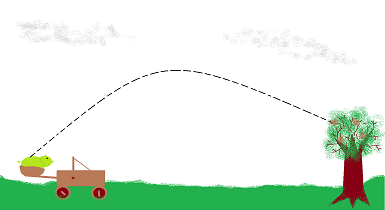
\includegraphics[width=12cm]{conceptsmall}
\end{center}

\chapter{Tehnologija}

\section{Generiranje dreves}
Problem generiranja primerno realističnih dreves se je izkazal za
algoritemsko precej zanimivega. V namene seminarske naloge je bil
rešen ``iz nule'', čeprav je ta problem že dokaj raziskan v obliki
L-sistemov in verjetno še česa. Ampak to ni tako zabavno.

Osnovna postavka merjenja uspeh akončnega algoritma je bila funkcijska
čistost, saj sem želel postaviti siste, ki iz peščice začetnih
podatkov generira neskončno število različnih dreves. Realističnost je
parameter, ki ga je bilo malo težje meriti zato je umetniški vtis
končnega rezultata bolj subjektivna ocena, da so drevesa uspešno
zgenerirana kot pa neka številka. Ako bi že moral definirati kako
uspešno algoritem generira drevesa, porečem, da 7.

\subsection{Osnovni princip}
Algoritem je zasnovan kot generator fraktalov, ki mu podamo nek vektor
in osnovno dolžino veje, ta pa potem rekurzivno kliče samega sebe,
dokler ne doseže neke smiselno določene meje globine drevesa.

Glavna funkcija algoritma se najprej odloči koliko vej je potrebnih na
trenutni globini, kar je definirano z vrsto praštevil (2,3,5
...). Nato izračuna vektorski produkt med podanim vektorjem V in nekim
izmišljenim vektorjem, s čimer dobi prvo vejo na trenutnem nivoju.

Ko je izbrana prva veja, jo samo (N-1)-krat duplicira in zavrti okrog
vektorja V. Tako ima osnovno vejo (vektor V) ter N nanjo pravokotnih
vej, ki predstavljajo poddrevo in so enakomerno razporejene po ravnini
na vrhu V.

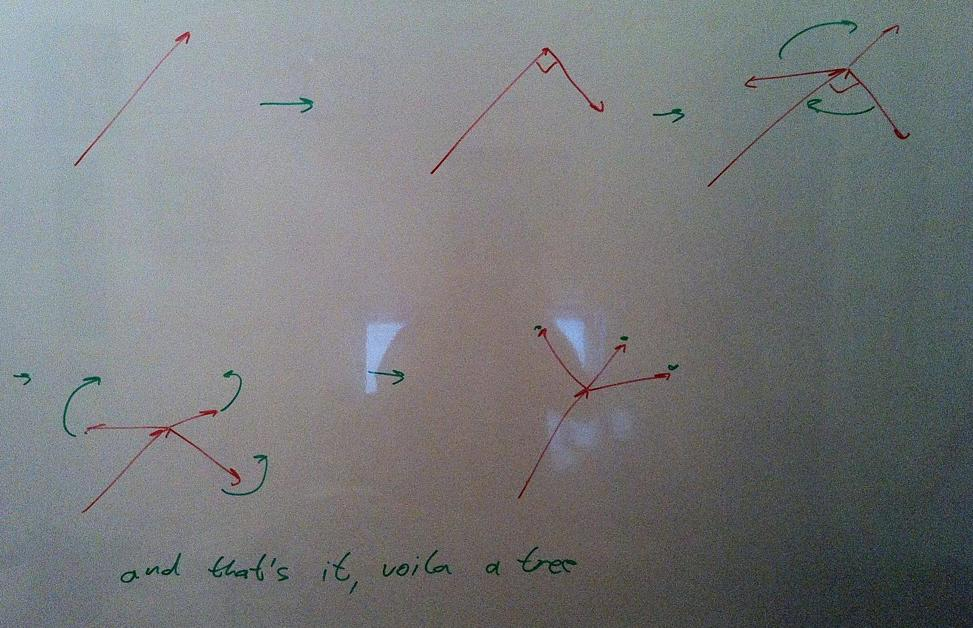
\includegraphics[width=12cm]{algorithmsketch.jpg}

Naslednji korak je samo še preprosta rotacija vseh vej za nek kot v
nasprotni smeri vektorja V in že imamo zgenerirano krošnjo za podano
vejo oz. deblo. Nato algoritem spet pokliče samega sebe na vrhu vsake
tako zgenerirane veje.


\subsection{Naključnost}
Po zgornjem algoritmu so drevesa sicer zgledala dokaj realistična,
vendar pa so bila vsa enaka, kar je bilo tako dolgočasno, kot je
onemogočalo, da bi tudi gozd deloval prilično resničen. Rešitev je
torej neka stopnja naključnosti.

Že intuitivno je opaziti, da drevo ne more biti popolnoma naključno,
saj potem izgubi na vsem kar ga sploh dela za drevo in postane samo
kup nekoherentnih črt. V interesu pravega znanstvenega pristopa in
izogibanja intuitivnim skokom logike, je bilo zgenerirano tudi eno
tako drevo.

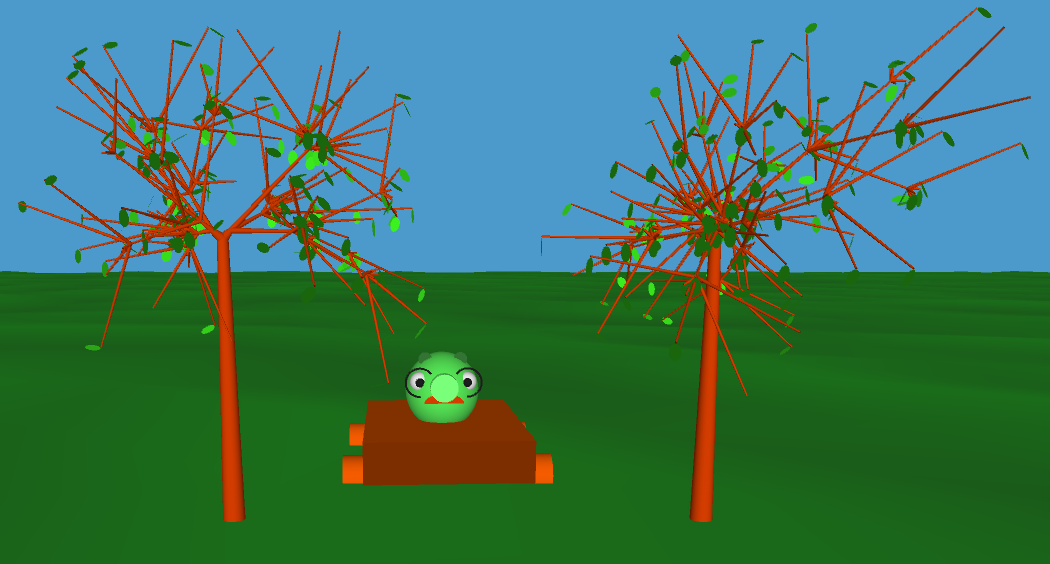
\includegraphics[width=12cm]{randomtree.png}

Naključnost je bilo zategadelj potrebno zapreti v neke smiselne
okvire, tako da bo algoritem sposoben generirati dovolj različnih
dreves, a bo vseeno vsakič zgeneriral drevo.

Podobno kot se osnoven algoritem izvaja v treh korakih, je tudi
naključnost dodana na tri osnovne načine.

Prva stopnja naključnosti se zgodi pri razporejanju vej po ravnini nad
osnovno vejo. Tu se pri vsaki rotaciji kotu preprosto doda nek
naključno izbran majhen kot v naključno smer, tako da razporeditev ni
čisto uniformna.

Druga stopnja naključnosti pride pri izbiri kota rotacije ``navzgor'',
ki določa kako široka bo krošnja. Tu gre za dokaj osnovno verzijo
uteženega naključnega izbiranja - algoritmu je namreč podan statično
izbran spisek deliteljev polnega radiana, tako da so naključne izbire
v končni fazi zgenerirale subjektivno zadvooljivo drevo. V končni
verziji kode ta del verjetno ne bo več tako statičen.

Najbolj zanimivo računanje naključnosti pa je pri izbiranju dolžine
vej, saj se je izkazalo za izredno pomembno, da so vse naslednje veje
krajše od prejšnjih, ter da se zelo kratke veje ne pripetijo prezgodaj
v drevesu. V ta namen je bila ustvarjena funkcija naključne izbire,
kateri lahko podamo funkcijo gostote verjetnosti. Na ta način
pridobimo popoln nadzor nad obliko verjetnosti.

Funkcija gostote verjetnosti, ki se je izkazala za najboljšo, je
zlepek, ki zagotavlja, da ima vsak naslednji nivo krajše veje od
prejšnjega, ter vsaki naslednji možni izbiri dolžine določi tretjino
verjetnosti prejšnje. (dolžine so namreč zaporedje vse manjših
večkratnikov osnovne dolžine, ki je parameter algoritma).

\subsection{Gravitacija}

\section{The rest}

\chapter{Rezultati}


\end{document}
